% Generated by render.py; edit preamble.tex, citations.json and main.tikz
\documentclass[border=12pt]{standalone}
\def\pgfsysdriver{pgfsys-dvisvgm.def}
\usepackage[dvisvgm]{xcolor}
\usepackage{xeCJK}
\setCJKmainfont{HaranoAjiGothic-Regular.otf}[BoldFont=HaranoAjiGothic-Bold.otf]
\setCJKsansfont{HaranoAjiGothic-Regular.otf}[BoldFont=HaranoAjiGothic-Bold.otf]
\usepackage{amsmath,amssymb,tikz,lmodern}
\usetikzlibrary{arrows.meta,positioning,calc,fit,backgrounds}
\renewcommand{\familydefault}{\sfdefault}
\definecolor{ink}{HTML}{25322F}
\definecolor{green}{HTML}{246657}
\definecolor{tint}{HTML}{EEF4F0}
\definecolor{soft}{HTML}{C6D2CC}
\definecolor{muted}{HTML}{52615B}
\newif\ifJapanese
\newcommand{\Tx}[2]{\ifJapanese #1\else #2\fi}
\newcommand{\Eff}{\overline{\operatorname{Eff}}}
\newcommand{\heading}[3]{{\color{green}\bfseries #1\quad\Tx{#2}{#3}}\\[5pt]}
% A white rectangle makes the complete citation label clickable, including spaces.
\newcommand{\refurl}[2]{\special{dvisvgm:raw <a xlink:href="#1" target="_blank" rel="noopener noreferrer">}{\setlength{\fboxsep}{0pt}\colorbox{white}{\color{green}\underline{\strut #2}}}\special{dvisvgm:raw </a>}}
\tikzset{
 card/.style={draw=soft,fill=white,rounded corners=2pt,align=left,text=ink,font=\fontsize{10.5}{14}\selectfont,inner xsep=12pt,inner ysep=10pt,text width=14.4cm},
 half/.style={card,text width=6.45cm,minimum height=2.05cm},
 result/.style={card,draw=green,fill=tint,line width=.9pt},
 reason/.style={align=left,text=muted,font=\fontsize{9}{12}\selectfont,inner sep=0pt,text width=12.6cm},
 branchreason/.style={reason,text width=5.95cm},
 edge/.style={-{Stealth[length=2.4mm]},draw=green,line width=1pt},
 wire/.style={draw=green,line width=1pt},
}
% Keep the arrow in a dedicated left gutter; explanations never cover it.
\def\flow#1#2#3;{
 \coordinate (#2-from) at ($(#1.south)+(-6.9,0)$);
 \coordinate (#2-to) at ($(#2.north)+(-6.9,0)$);
 \draw[edge] (#2-from)--(#2-to);
 \node[reason,anchor=west] (#2-reason) at ($(#2-from)!.5!(#2-to)+(.55,0)$) {#3};
}

% Style adapted from the repository's Schnell diagrams; MIT attribution retained.

% Generated from citations.json; do not edit.
\newcommand{\Cite}[1]{\csname cite-#1\endcsname}
\expandafter\def\csname cite-main\endcsname{\shortstack[l]{\refurl{https://github.com/openai/math/blob/1581d4cbdd69a0faf34b2089614fe2a814316a6a/preprints/Minimal-models-in-numerical-dimension-one-September-24-2026/paper.pdf}{Theorem 1.1; equation (1.1) · pp. 1–2}}}
\expandafter\def\csname cite-cor\endcsname{\shortstack[l]{\refurl{https://github.com/openai/math/blob/1581d4cbdd69a0faf34b2089614fe2a814316a6a/preprints/Minimal-models-in-numerical-dimension-one-September-24-2026/paper.pdf}{Corollary 1.2 · p. 2}}}
\expandafter\def\csname cite-perturbations\endcsname{\shortstack[l]{\refurl{https://github.com/openai/math/blob/1581d4cbdd69a0faf34b2089614fe2a814316a6a/preprints/Minimal-models-in-numerical-dimension-one-September-24-2026/paper.pdf}{Proposition 2.1; Lemmas 2.2–2.3 · pp. 4–8}}}
\expandafter\def\csname cite-growth\endcsname{\shortstack[l]{\refurl{https://github.com/openai/math/blob/1581d4cbdd69a0faf34b2089614fe2a814316a6a/preprints/Minimal-models-in-numerical-dimension-one-September-24-2026/paper.pdf}{Lemma 3.1 · pp. 8–10}}}
\expandafter\def\csname cite-nefness\endcsname{\shortstack[l]{\refurl{https://github.com/openai/math/blob/1581d4cbdd69a0faf34b2089614fe2a814316a6a/preprints/Minimal-models-in-numerical-dimension-one-September-24-2026/paper.pdf}{Lemmas 3.2–3.3; Proposition 3.4 · pp. 10–13}}}
\expandafter\def\csname cite-completion\endcsname{\shortstack[l]{\refurl{https://github.com/openai/math/blob/1581d4cbdd69a0faf34b2089614fe2a814316a6a/preprints/Minimal-models-in-numerical-dimension-one-September-24-2026/paper.pdf}{Section 4; equation (4.1) · pp. 13–14}}}
\expandafter\def\csname cite-comparison\endcsname{\shortstack[l]{\refurl{https://github.com/openai/math/blob/1581d4cbdd69a0faf34b2089614fe2a814316a6a/preprints/Minimal-models-in-numerical-dimension-one-September-24-2026/paper.pdf}{Proposition 2.1(iii); Lemma 2.2 · pp. 4–5, 8}}}
\expandafter\def\csname cite-bchm\endcsname{\shortstack[l]{\refurl{https://arxiv.org/pdf/math/0610203v2\string##page=10}{[BCHM10, Corollary 1.4.2, p. 10]}}}
\expandafter\def\csname cite-laz\endcsname{\shortstack[l]{\refurl{https://www.math.stonybrook.edu/~roblaz/Reprints/Lazarsfeld.PCMI.Short.Course.MI.pdf\string##page=11}{[Laz10, Theorem 2.4, p. 11]}}}
\expandafter\def\csname cite-la\endcsname{\shortstack[l]{\refurl{https://github.com/openai/math/blob/1581d4cbdd69a0faf34b2089614fe2a814316a6a/preprints/Log-abundance-in-characteristic-zero-September-24-2026/paper.pdf}{[OpenAI26LA, Theorem 1.1, p. 2]}}}

\Japanesetrue
\begin{document}
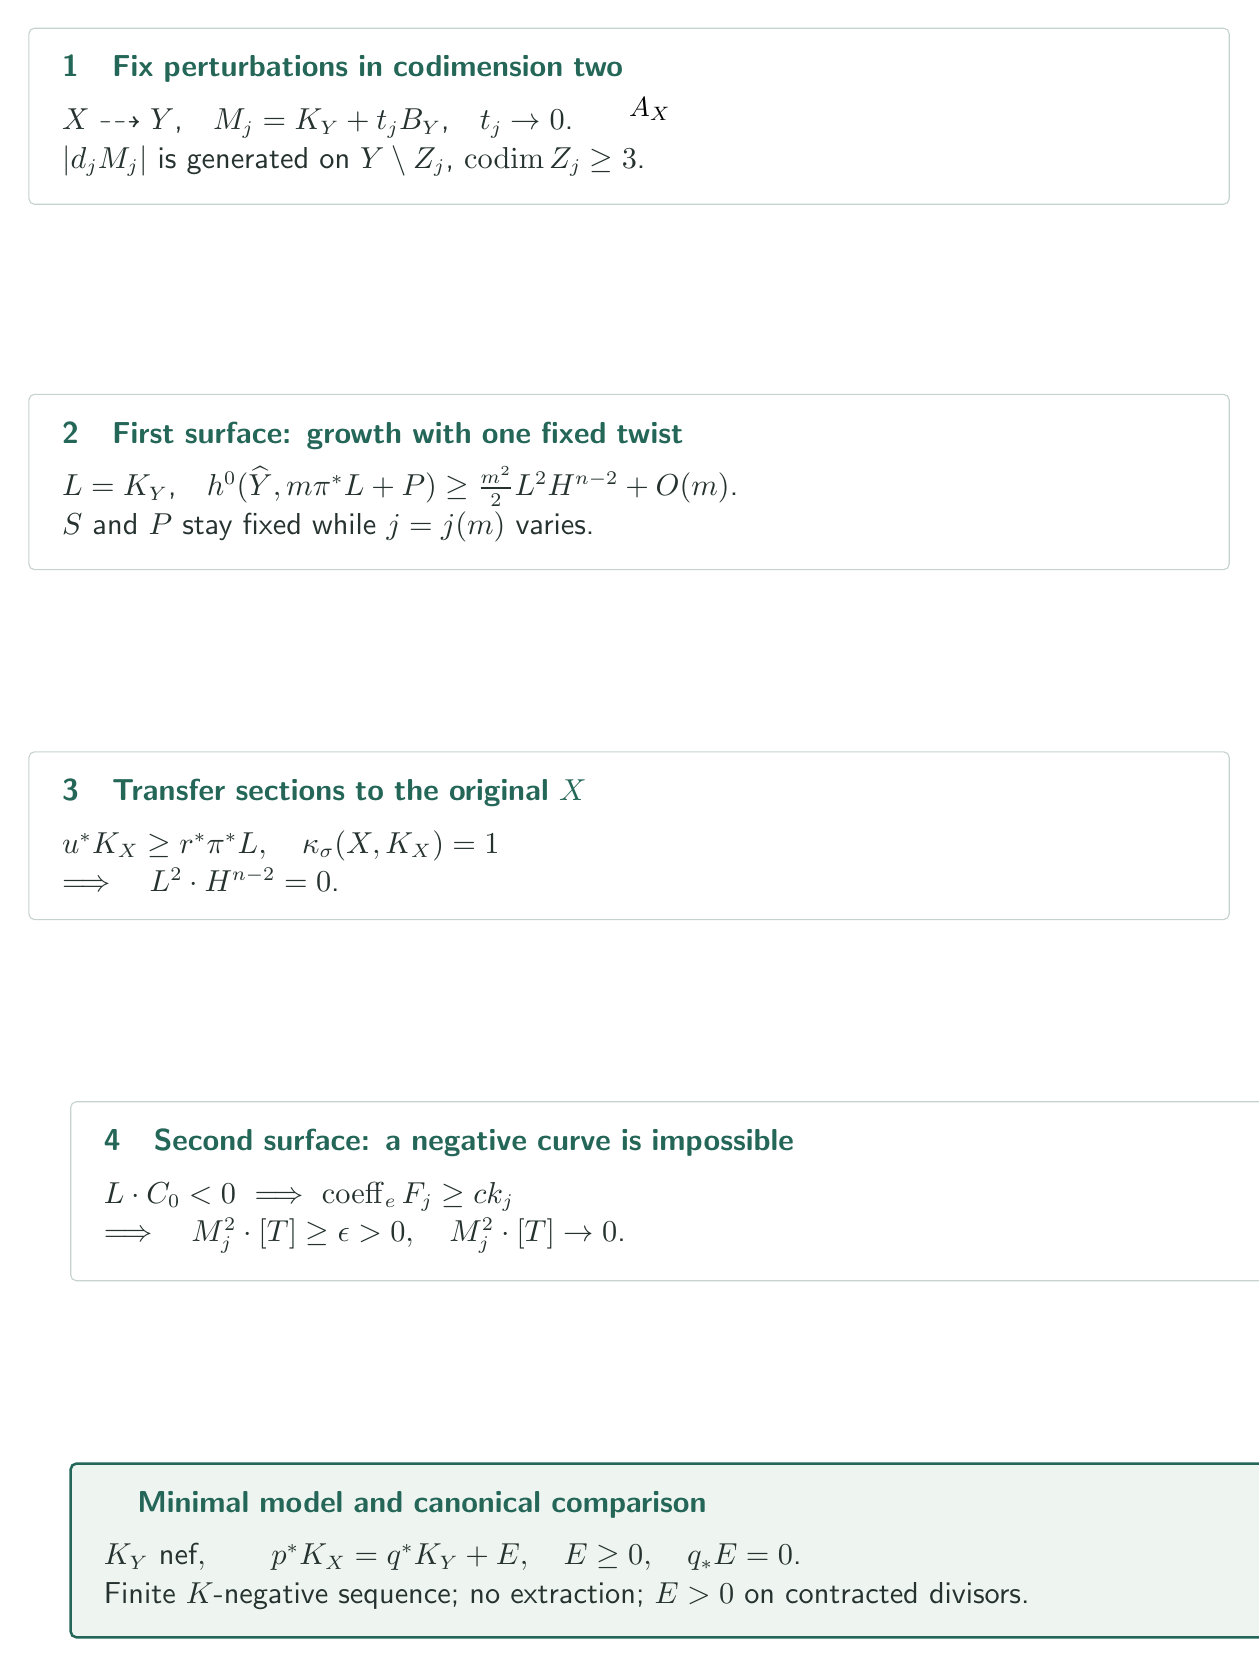
\begin{tikzpicture}
\node[card] (a) {\heading{1}{正摂動を余次元2で固定}{Fix perturbations in codimension two}
$X\dashrightarrow Y$,\quad $M_j=K_Y+t_jB_Y$,\quad $t_j\to0$.\\
\Tx{$|d_jM_j|$は$Y\setminus Z_j$で生成、$\operatorname{codim}Z_j\geq3$。}{$|d_jM_j|$ is generated on $Y\setminus Z_j$, $\operatorname{codim}Z_j\geq3$.}};
\node[card,below=2.4cm of a] (b) {\heading{2}{第一の曲面：固定捻りの二次増大}{First surface: growth with one fixed twist}
$L=K_Y$,\quad $h^0(\widehat Y,m\pi^*L+P)\geq\frac{m^2}{2}L^2H^{n-2}+O(m)$.\\
\Tx{$j=j(m)$を選んでも$S,P$は固定する。}{$S$ and $P$ stay fixed while $j=j(m)$ varies.}};
\flow a b {\Tx{Nadel消滅とKoszul複体で制限を全射にする}{Nadel vanishing and Koszul give surjective restriction}\\\Cite{growth}\quad\Cite{laz}};
\node[card,below=2.3cm of b] (c) {\heading{3}{元の$X$へ切断を移す}{Transfer sections to the original $X$}
$u^*K_X\geq r^*\pi^*L,\quad \kappa_\sigma(X,K_X)=1$\\
$\Longrightarrow\quad L^2\cdot H^{n-2}=0$.};
\flow b c {\Tx{一つのample $A_X$で正の二次limsupを排除}{One ample $A_X$ excludes positive quadratic limsup}\\\Cite{completion}};
\node[card,below=2.3cm of c] (d) {\heading{4}{第二の曲面：負の曲線は矛盾}{Second surface: a negative curve is impossible}
$L\cdot C_0<0\ \Longrightarrow\ \operatorname{coeff}_eF_j\geq ck_j$\\
$\Longrightarrow\quad M_j^2\cdot[T]\geq\epsilon>0,\quad M_j^2\cdot[T]\to0$.};
\flow c d {\Tx{固定した点・例外曲線でjetとHodge indexを使う}{Jets and Hodge index on a fixed point and exceptional curve}\\\Cite{nefness}};
\node[result,below=2.3cm of d] (e) {\heading{}{極小モデルと標準因子の比較}{Minimal model and canonical comparison}
$K_Y\text{ nef},\qquad p^*K_X=q^*K_Y+E,\quad E\geq0,\quad q_*E=0$.\\
\Tx{有限$K$-negative列、因子非抽出、縮約因子上で$E>0$。}{Finite $K$-negative sequence; no extraction; $E>0$ on contracted divisors.}};
\flow d e {\Tx{nef性に、有限prefixのdiscrepancy比較を合わせる}{Combine nefness with discrepancies of the finite prefix}\\\Cite{comparison}};

\end{tikzpicture}
\end{document}
